% !TeX spellcheck = en_GB
\documentclass[10pt,letterpaper,oneside]{article}
\def\NoteAuthor{Andreas Stöckel and Chris Eliasmith}
\usepackage{fontspec}
\usepackage{arev}
\usepackage[utf8]{inputenc}
\usepackage[T1]{fontenc}
\usepackage{amsmath}
\usepackage{amsfonts}
\usepackage{amssymb}
\usepackage{graphicx}
\usepackage{csquotes}
\usepackage{booktabs}
\usepackage{multicol}
\usepackage{enumerate}
\usepackage{microtype}
\usepackage[labelfont=bf,font={small}]{caption}
\usepackage{hyperref}
\usepackage{booktabs}
\usepackage{subcaption}
\usepackage{fancyhdr}
\usepackage[svgnames]{xcolor}
\usepackage{mdframed}
\usepackage{multicol}
\usepackage[para]{footmisc}
\usepackage{siunitx}
\usepackage{cleveref}
\usepackage{listings}
\usepackage{cprotect}


\lstset{ % General setup for the package
	language=Python,
	basicstyle=\small\ttfamily,
	tabsize=4,
	columns=fixed,
	showstringspaces=false,
	showtabs=false,
	keepspaces,
	commentstyle=\color{SeaGreen},
	keywordstyle=\bf\ttfamily\color{DarkBlue},
	stringstyle=\ttfamily\color{Crimson}
}

\newfontfamily\symbolfont{Symbola}
\usepackage[left=1in,right=1in,top=1in,bottom=1in,marginparwidth=0.3in]{geometry}

\usepackage[sorting=none]{biblatex}
\addbibresource{../bibliography.bib}

\ifx\NoteAuthor\undefined
  \def\NoteAuthor{Andreas Stöckel and Chris Eliasmith}
\fi

\ifx\BasedOn\undefined
  \def\BasedOn{Based on lecture notes by\\Chris Eliasmith and Terrence~C.~Stewart}
\fi

\author{\NoteAuthor\\[0.5cm]\BasedOn}
\newcommand{\baseCodeURL}{https://github.com/celiasmith/syde556-f23/blob/master/lectures}

\fancyhf{}
\fancyhead[L]{SYDE 556/750 Lecture Notes}
\fancyhead[R]{\NoteAuthor}
\fancyfoot[C]{\thepage}
\pagestyle{fancy}

\setlength{\parindent}{0em}
\setlength{\parskip}{0.5em}
\renewcommand{\baselinestretch}{1.25}

\renewcommand{\vec}[1]{{\mathbf{#1}}}
\newcommand{\mat}[1]{{\mathbf{#1}}}
\newcommand{\T}{\ensuremath{\mathrm{T}}}
\renewcommand{\epsilon}{\varepsilon}
\renewcommand{\phi}{\varphi}

\makeatletter
\newcommand{\superimpose}[2]{%
	{\ooalign{{#1}\hidewidth\cr{#2}\hidewidth\cr}}}
\makeatother
\newcommand{\SolidCircle}[2]{\superimpose{\color{#1}\symbolfont ⬤}{\textbf{\color{white}#2}}\hspace{1em}}
\newcommand{\OPlus}{\SolidCircle{DarkGreen}{\kern0.75pt+}}
\newcommand{\OMeh}{\SolidCircle{DarkOrange}{~}}
\newcommand{\OMinus}{\SolidCircle{DarkRed}{\kern2.25pt--}}

\newcommand{\YouTube}[2][Video]{\href{https://youtu.be/#2}{{\symbolfont 📺}~{#1}}%
%\footnote{\url{https://youtu.be/#2}}%
}

\newcommand{\CodeLink}[2][Code]{\href{\baseCodeURL/#2}{{\symbolfont ⌨}~\emph{#1}}}

\newcommand{\MakeTitle}[1]{
\maketitle
\begin{center}
	
\includegraphics[width=0.5\textwidth]{../assets/uwlogo.pdf}\\[1cm]
	{#1}\
\end{center}

\vfill

\thispagestyle{empty}
\setcounter{page}{0}
\newpage

\pagenumbering{roman}
\setcounter{tocdepth}{2}
\tableofcontents
\newpage

\setcounter{page}{0}
\pagenumbering{arabic}}

\reversemarginpar


\newcommand{\ColorBox}[3]{%
	\marginpar{%
		\huge\raisebox{-3ex}{\symbolfont{#1}}%
	}%
	\begin{mdframed}[hidealllines=true,backgroundcolor=#2,innertopmargin=0.25cm,innerbottommargin=0.25cm]%
		{#3}
	\end{mdframed}}

\newcommand{\Note}[1]{\ColorBox{📌}{WhiteSmoke}{\textbf{Note:} #1}}
\newcommand{\Example}[1]{\ColorBox{💡}{WhiteSmoke}{\textbf{Example:} #1}}
\newcommand{\Aside}[1]{\ColorBox{🌟}{WhiteSmoke}{\emph{Aside:} #1}}
\newcommand{\Python}[1]{\ColorBox{🐍}{WhiteSmoke}{#1}}
\newcommand{\Notation}[1]{\ColorBox{\huge$\Sigma$}{WhiteSmoke}{\textbf{Notaton:} #1}}

\newcommand{\ConstructionSite}{\hrulefill {\symbolfont 🚧} UNDER CONSTRUCTION {\symbolfont 🚧} \hrulefill}

\newenvironment{ImportantEqn}[1]{\mdframed\raggedleft\emph{({#1})}\align}{\endalign\endmdframed}

\date{November 17 \& 18, 2022}
\title{SYDE 556/750 \\ Simulating Neurobiological Systems \\ Lecture 11: The Semantic Pointer Architecture}

\newcommand{\Pred}[1]{\ensuremath{\mathbf{\textcolor{Crimson}{#1}}}}
\newcommand{\Obj}[1]{\ensuremath{\mathtt{\textcolor{RoyalBlue}{#1}}}}
\newcommand{\Fun}[1]{\ensuremath{\mathit{\textcolor{ForestGreen}{#1}}}}
\newcommand{\CC}{\circledast}

\begin{document}

\MakeTitle{\textbf{Accompanying Readings: Chapter 3, 5, 6 and 7 of \enquote{How to Build a Brain}}}

\section{Introduction}

\Note{In the previous lecture, we discussed Vector Symbolic Algebras (VSAs) in combination with circular convolution as a way to represent symbols as vectors and to \enquote{combine} concepts into a new one. However, VSAs alone are not a \enquote{cognitive architecture}. It is unclear how to build \enquote{cognitive agents} that receive information from the environment, turn this information into symbol vectors, and finally produce \emph{behaviour}. The semantic pointer architecture (SPA) is an attempt at providing a cognitive architecture combining VSAs, the NEF, and other modeling approaches to produce \emph{biological cognition}.}

As we have seen, we can use Vector Symbolic Algebras in conjunction with circular convolution to solve some relatively challenging cognitive problems, such as Raven's progressive matrices. Furthermore, we can use the NEF to implement such approaches in spiking neural networks. However, so far, we have presumed that a certain vocabulary of random symbol vectors exists and that there is some kind of system in place that extracts these symbol vectors from the environment.

In this lecture we are going to be a little more specific. We are going to describe an NEF-implementable architecture based on symbol vectors that hypothesises how sensory information could be turned into symbol vectors, how these vectors are processed, and, lastly, how symbol vectors can be turned into motor commands. This architecture is called the \enquote{Semantic Pointer Architecture} (SPA).

At a smaller scale, the SPA can be used to build neural models of cognitive phenomena such as working memory or language association tasks. At a larger scale, the SPA has been used to build the largest functional brain model to date, the Semantic Pointer Architecture Unified Network (Spaun) \cite{eliasmith2012largescale,choo2018spaun}. Spaun is able to solve a variety of cognitive tasks, using the same underlying spiking neural network and without being \enquote{reprogrammed}. This ability is a major strength of the SPA in contrast to other models of cognition.

In this lecture we will first have a broader look at the SPA. In the book \enquote{How to build a brain}, the SPA is broken down into chapters on semantics, syntax, control, and learning and memory. We have already seen how syntax is handled, as the SPA uses a spiking implementation of circular convolution.  We have also seen examples of learning in earlier lectures that are quite similar to the methods in the SPA. In this lecture we will focus on the other elements of the SPA, starting with the concepts of \enquote{shallow and deep semantics}. Then, we have quick look at Spaun, and in particular a specific model of human serial working memory, followed by a discussion of cognitive control and action selection in particular.

\section{The Semantic Pointer Architecture}

\Note{The content of this section is to a large degree based on Chapter 3 of \enquote{How to Build a Brain} \cite{eliasmith2013how}. Read the chapter for a more thorough discussion of semantic pointers.}

In a nutshell, the Semantic Pointer Architecture combines the ideas of Vector Symbolic Algebras (VSAs), deep convolutional neural networks, control theory, and action selection all while using the NEF as a \enquote{neural compiler}. In addition, the SPA adopts a specific cognitive architecture---the basal ganglia cortex control loop.

Given the overall architecture, symbol vectors in the SPA are no longer random, but thought to be the result of a partly reversible \emph{compression} process. Just as a pointers in most programming languages can be \enquote{dereferenced} to access the original content, symbol vectors $\vec x$ constructed in this way can be \emph{decompressed} to access the information---\enquote{deep semantics}---about the underlying represented object. Hence, symbol vectors in the SPA are called \emph{semantic pointers}.

The SPA argues for the Semantic Pointer Hypothesis. Simply put, this hypothesis states: 
\begin{quote}
Higher-level cognitive functions in biological systems are made possible by semantic pointers. Semantic pointers are neural representations that carry partial semantic content and are composable into the representational structures necessary to support complex cognition.
\end{quote}


\subsection{Shallow and Deep Semantics}

In order to gain a better understanding of semantic pointers, we must first distinguish between \enquote{shallow} and \enquote{deep} semantics. The difference between the two can best be explained by what artificial intelligence researchers refer to as the \enquote{symbol grounding problem}.

In general---and without going into any philosophical details---a \emph{symbol} is an arbitrary mapping from a short piece of information (the representation of the symbol itself) onto a richer semantic concept.

For example, consider the symbol {\Obj{TREE}}. As a human being seeing this symbol, we tend to immediately map it onto a certain class of tall plants, along with the corresponding visual imagery, smells, sounds, and textures. All this cross-modal information establishes the \emph{deep semantics} of the symbol, i.e.,~our \enquote{experience} of the concept.

Now consider an early 1980s artificial intelligence researcher building a symbolic reasoning system. In such a system the symbol {\Obj{TREE}} might just be represented as a short sequence of bytes (i.e., \Obj{TREE} is \texttt{0x54 0x52 0x45 0x45} in ASCII), along with a set of similarly encoded information linking this symbol to other symbols, for example
\begin{align*}
	\forall x \Pred{is\_a}(x, \Obj{PINE}) &\rightarrow \Pred{is\_a}(x, \Obj{TREE}) \wedge \Pred{has}(x, \Obj{NEEDLES}) \wedge \Pred{is}(x, \Obj{EVERGREEN}) \,, \\
	\forall x \Pred{is\_a}(x, \Obj{TREE}) &\rightarrow \Pred{is\_a}(x, \Obj{PLANT}) \,, \quad \forall x \Pred{is\_a}(x, \Obj{PLANT}) \rightarrow \Pred{is}(x, \Obj{ALIVE}) \,.
\end{align*}
The problem of \enquote{symbol grounding} is the observation that even though we could imagine building a database with all important information there is to know about a concept, the symbols we use in this relational description (the \emph{shallow semantics}) are not really linked or related to any sensory information or \enquote{experience} of the world.

\Aside{A project that aims to build exactly such a database is Douglas Lenat's Cyc project, started in 1984. The database is still under active development. (\url{https://www.cyc.com/})}

The random symbol vectors we discussed in the last lecture are as arbitrary a mapping onto concepts as the relationship between the byte sequence \texttt{0x54 0x52 0x45 0x45} and an actual tree. Such vectors will thus at most be useful for \emph{shallow} semantics. This is similarly true for some non-random methods deriving symbol vectors.

One example of such methods are \emph{word embeddings}. Here, the general idea is to perform some statistical analysis of how often certain words appear closely together in large corpora of text, usually resulting in a term-frequency matrix. One can then apply a dimensionality reduction method (such as PCA or auto-encoders) to this data, mapping each word onto a vector with a few hundred dimensions.

Interestingly, such mappings capture relational semantics of the represented concepts. For example, using the \enquote{word2vec} embedding \cite{mikolov2013efficient}, we can perform the following arithmetic\footnote{See \url{http://turbomaze.github.io/word2vecjson/} for an online demo. Ignore concepts in the output that are already present in your input.}:
\begin{align*}
	\Obj{WOMAN} + (\Obj{KING} - \Obj{MAN}) &\approx \Obj{QUEEN} \,,\\
	\Obj{SPACE} + (\Obj{SHIPS} - \Obj{WATER}) &\approx \Obj{SPACESHIP} \,.
\end{align*}
While these embeddings are great as part of VSAs, they do not capture any \enquote{deep semantics}.

\begin{figure}[p]
	\centering
	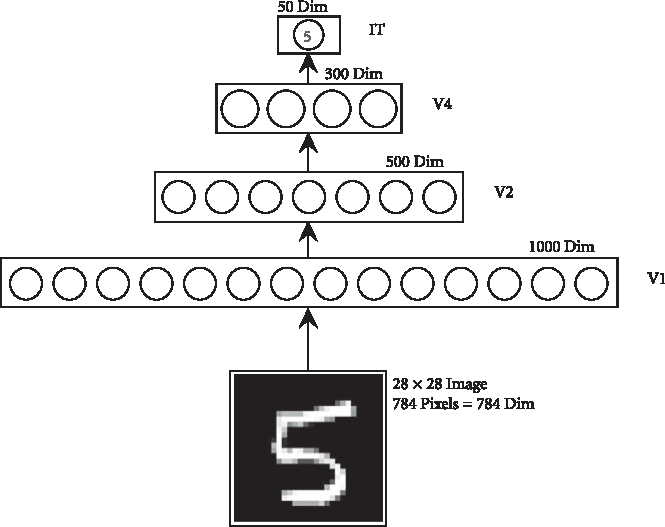
\includegraphics[scale=1.15]{media/htbab_hierarchy.pdf}
	\caption{Visual processing hierarchy. The representation in the uppermost layer corresponds to a semantic pointer. Notice that there is a direct relationship between the input and the representation. Changing the visual stimulus (i.e., different styles of \enquote{fives}) will be captured in the final representation. Figure copied from Eliasmith, \enquote{How to build a brain}, 2013, Figure 3.4.}
	\label{fig:htbab_hierarchy}
\end{figure}

\begin{figure}[p]
	\centering
	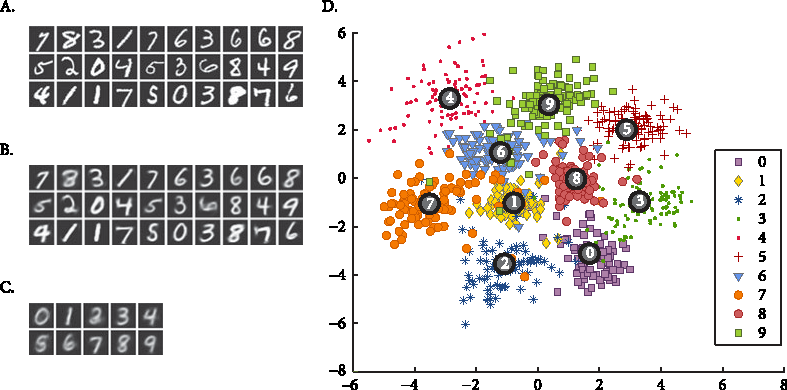
\includegraphics[scale=1.15]{media/htbab_dereference.pdf}
	\caption{Dereferencing semantic pointers. \textbf{A.} Original input images. \textbf{B.} \enquote{Dereferenced} semantic pointers. \textbf{C.} Dereferenced average semantic pointer. \textbf{D.} Dimensionality reduction of the 50-dimensional semantic pointer space. Figure copied from Eliasmith, \enquote{How to build a brain}, 2013, Figure 3.7.}
	\label{fig:htbab_dereference}
\end{figure}

\subsection{Deep Semantics for Perception}

Now, how are semantic pointers supposed to capture parts of the \enquote{deep semantics} of objects? As mentioned above, the answer is that semantic pointers are thought to be generated by repeated compression of stimuli, i.e., the symbol is directly related to the stimulus it represents.

As an example, take vision: we know that visual stimuli are processed in multiple \enquote{layers} of visual cortex, where the complexity of the represented concepts increases with each layer (V1, V2, V4, IT). In other words, each layer is performing dimensionality reduction (or compression) of the information in the previous layer, trying to extract as much information as possible from the previous layer (\cref{fig:htbab_hierarchy}).

The representation in the \enquote{final} layer could be interpreted as a \emph{semantic pointer}. Notice that this vectorial representation is directly influenced by the input to the system. Changes to the visual stimulus will result in slightly different representations. Crucially, we can \enquote{dereference} or \enquote{decompress} the visual representation. That is, we can \enquote{clamp} the final layer to a specific semantic pointer and compute in \enquote{backwards direction} which neural activity is most likely to evoke a certain semantic pointer (\cref{fig:htbab_dereference}). In the context of visual processing, this would correspond to \enquote{mental imagery}.

\subsection{Deep Semantics for Action}

\begin{figure}
	\centering
	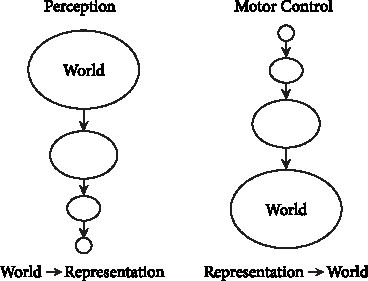
\includegraphics{media/htbab_perceptual_motor.pdf}
	\caption{Perception and action can be described as similar, but reversed processes. Perception compresses a high-dimensional signal from the environment into a low-dimensional description, a semantic pointer. Motor-control decompresses a semantic pointer into a high-dimensional motor plan (i.e., muscle tensions over time). Figure copied from Eliasmith, \enquote{How to build a brain}, 2013, Figure 3.9.}
\end{figure}

Similar processing hierarchies do not only exist for visual perception, or, perception in general. For example, there is evidence that high-level motor commands are successively being translated into more detailed control signals. In a sense, this is exactly the opposite problem of turning a high-dimensional perceptual signal into a low-dimensional semantic pointer. 

We can treat these high-level control signals as \enquote{semantic pointers} that are being decompressed into a high-dimensional control signal (i.e., all possible muscle tensions in the body over time). Correspondingly, a semantic pointer for motor control might be something such as \enquote{reach the bottle} (represented in cortical areas such as the pre-motor area \enquote{PM} and the supplemental motor area \enquote{SMA}), which is then turned into a detailed motor plan (in cortical areas such as M1, S1, and S2 in conjunction with non-cortical areas such as the cerebellum).

\Note{A model that implements optimal motor control on top of this framework is the \enquote{NOCH} model by Travis Dewolf \cite{dewolf2010nocha}. This model is also described in Chapter 3 of \enquote{How to Build a Brain}.}

\subsection{Using the Semantic Pointer Architecture in Nengo}

\begin{figure}
	\centering
	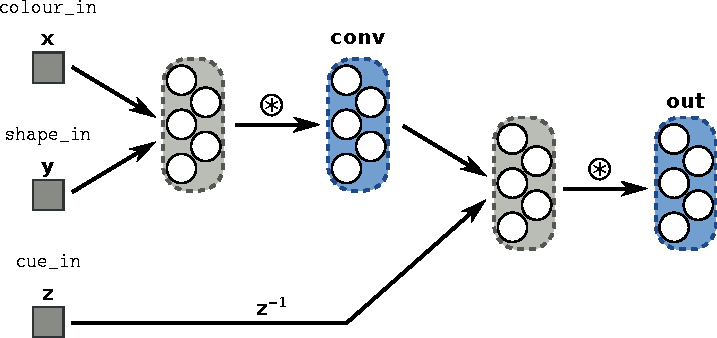
\includegraphics{media/spa_network.pdf}
	\caption{Network diagram of the SPA example network performing \enquote{question answering} described below. Grey boxes correspond to input nodes (\enquote{\texttt{spa.Transcode}} objects), large boxes to neuron populations. Grey neuron populations are implicitly generated by \texttt{nengo\_spa} in order to compute the circular convolution---as we have seen before, when computing multiplication (which is part of the circular convolution operator), both operands need to be represented in a common pre-population.}
	\label{fig:spa_network}
\end{figure}

In order to use semantic pointers in Nengo models, we can use the \texttt{nengo\_spa} library.\footnote{The current library to use is \texttt{nengo.spa} as \texttt{nengo\_spa} is being deprecated.} While this library does not implement the perception and action systems we discussed above (i.e., per default, semantic vectors are just random symbol vectors), it does provide an implementation of the action selection system we discuss below.

In a nutshell, the \texttt{nengo\_spa} library provides \texttt{spa.Transcode} in lieu of \texttt{nengo.Node} objects whenever a symbolic stimulus is received from the environment. Furthermore, \texttt{nengo.Ensemble} instances can be replaced with \texttt{spa.State} objects to represent symbol vectors in a neural population.

Consider the \enquote{question answering} example we discussed in the last lecture, where we saw that the pseudo-inverse of a symbol vector $\vec x$ can be used to reconstruct which other concept $\vec x$ has been bound to. For example, $(\Obj{RED} \CC \Obj{SQUARE}) \CC \Obj{SQUARE}^{-1} \approx \Obj{RED}$, i.e., we are asking the question \enquote{what property does the square have}?

The following code example (\CodeLink{lecture_11/media/code/spa.ipynb}) shows how to implement a network that queries different properties from a dynamically changing set of inputs. A diagram giving a better overview of what we are implementing here is given in \cref{fig:spa_network}.
\pagebreak\vspace*{-0.75cm}
\cprotect\Python{\begin{lstlisting}[language=python,morekeywords=with]
import nengo
import nengo_spa as spa

# Alternate between RED and BLUE as a color
def colour_input(t):
    if (t // 0.5) % 2 == 0:
        return "RED"
    else:
        return "BLUE"

# Alternate between CIRCLE AND SQUARE
def shape_input(t):
    if (t // 0.5) % 2 == 0:
        return "CIRCLE"
    else:
        return "SQUARE"

# Alternate between any of the four properties as a question/cue
def cue_input(t):
    sequence = ["0", "CIRCLE", "RED", "0", "SQUARE", "BLUE"]
    idx = int((t // (1. / len(sequence))) % len(sequence))
    return sequence[idx]

model = spa.Network()
dimensions = 32

with model:
    colour_in = spa.Transcode(colour_input, output_vocab=dimensions)
    shape_in = spa.Transcode(shape_input, output_vocab=dimensions)
    cue = spa.Transcode(cue_input, output_vocab=dimensions)    

    conv = spa.State(dimensions)
    out = spa.State(dimensions)

    # Connect the buffers using overloaded Python operators
    colour_in * shape_in >> conv
    conv * ~cue >> out
\end{lstlisting}}

\begin{figure}
	\centering\hspace*{-0.33cm}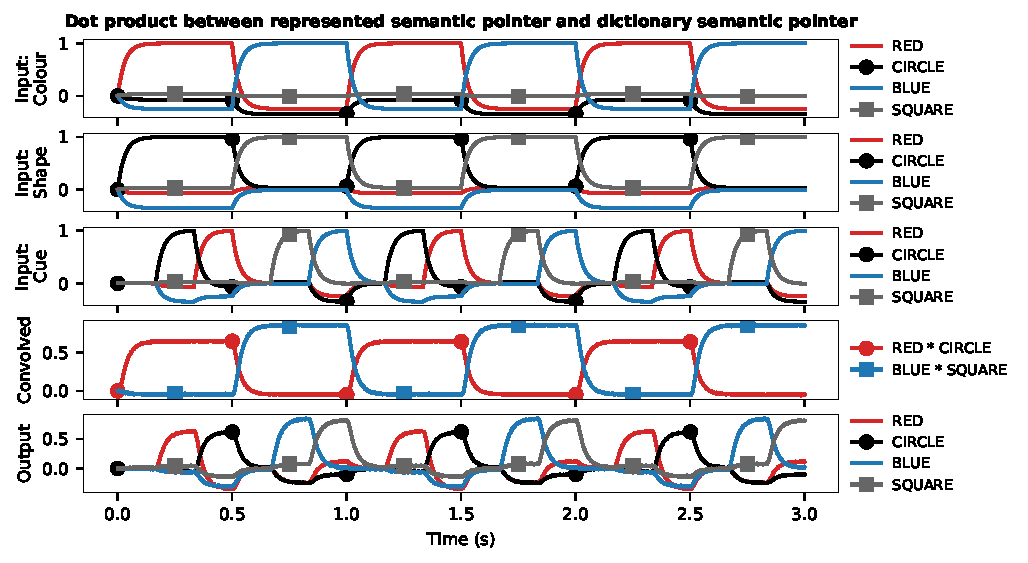
\includegraphics{media/nengo_spa_example.pdf}
	\caption{Output of the \texttt{nengo\_spa} \enquote{question answering} example detailed above. As can be seen in the output plot, the network correctly identifies the concept that is bound to any given cue. \CodeLink{lecture_11/media/code/spa.ipynb}}
	\label{fig:nengo_spa_example}
\end{figure}

Note that the strings returned in the callback functions passed to \texttt{spa.Transcode} are automatically translated into unique, randomly generated symbol vectors, the so called \enquote{vocabulary} of the model. \Cref{fig:nengo_spa_example} shows the result of running the above code. Since it is hard to visualise higher-dimensional vectors, the plots show the similarity of any vector currently represented in a population to the vectors in the vocabulary.

\Note{While the \texttt{nengo\_spa} library offers useful abstractions for building SPA models, keep in mind that the resulting network is still a low-level NEF network; even though you use the \texttt{spa.Transcode} or \texttt{spa.State} objects, the network is consisting of \texttt{nengo.Node} objects for anything input/output related and \texttt{nengo.Ensemble} objects for everything else.}

\section{Control: Action Selection}

\Note{The following sections are under construction and only outline information on the contents covered in class.}

To this point we have seen methods that allow us to construct and manipulate symbol-like information.  However, brains need to know \emph{when} to perform such manipulations.  This is the purpose of an action selection mechanism.  Action selection is one of two elements of control in the SPA. The other is \emph{routing}. `Routing' refers to ensuring that the right information goes to the right place at the right time. Selected actions are essentially implemented by routing. In what follows we consider both together, but focus on action selection.  A greater focus on routing would occur if we were discussing notions like `attention'.

\paragraph{What is an action?}
\begin{itemize}
	\item Physical movements (most obvious)
	\item Cognitive actions (less obvious), like
	\begin{itemize}
    \item Moving attention
    \item Changing the contents of working memory
    \item Recalling items from long-term memory
  \end{itemize}
	\item[$\Rightarrow$] Routing information in a particular way
\end{itemize}

Action selection is picking which of these to do.

\paragraph{Basal Ganglia}
Notes, do not write down!
\begin{itemize}
	\item All of cortex connects to this
	\item Output goes to Thalamus, central routing system
	\item Clinical evidence
	\begin{itemize}
		\item Parkinson's disease
		\begin{itemize}			
			\item Neurons in the substantia nigra die off
			\item Extremely difficult to trigger actions to start
			\item Usually physical actions; as disease progresses and more of the SNc is gone, can get cognitive effects too
			
		\end{itemize}
		\item Huntington's disease
		
		\begin{itemize}
			\item Neurons in the striatum die off
			\item Actions are triggered inappropriately (disinhibition)
			\item Small uncontrollable movements
			\item Trouble sequencing cognitive actions too
		\end{itemize}
	\end{itemize}
	\item Neurophysiological Evidence that BG are involved in RL, dopamine levels in BG correspond to reward prediction error
	\item Thalamus disinhibits other brain regions
	\item I.e., outputs $[1, 1, 0, 1]$ if action \textbf{C} is chosen
	\item Use inhibitory connections to suppress information from being transmitted
\end{itemize}

\paragraph{A simple example}
\begin{itemize}
	\item A critter is trying to survive in a harsh environment
	\item Possible actions
	\begin{itemize}
		\item[\textbf{A}] Go home
		\item[\textbf{B}] Move randomly
		\item[\textbf{C}] Go towards food
		\item[\textbf{D}] Go away from predator
	\end{itemize}
	\item Which one do we pick?
	\item[$\Rightarrow$] Reinforcement learning is a standard approach
\end{itemize}

\paragraph{Reinforcement Learning}
\begin{itemize}
	\item Learn function $Q(\vec s, \vec a)$ assigning a \emph{utility} to the current state
	\item Policy: choose action $\vec a$ with the highest utility $Q(\vec s, \vec a)$ in a given state $\vec s$ - i.e. use a selector like the BG to pick the action based on the value
\end{itemize}

\paragraph{Action Selection Examples}

We can try using lateral/mutual inhibition as in the code below.

\cprotect\Python{\begin{lstlisting}[language=python,morekeywords=with]
import nengo

def stimulus(t):
    if t<.3:
        return [.5,.4]
    elif .3<t<.5:
        return [.3,.5]
    else:
        return [0,0] 
    
model = nengo.Network('Selection')

with model:
    stim = nengo.Node(stimulus)
        
    s = nengo.Ensemble(200, dimensions=2)
    Qs = nengo.networks.EnsembleArray(50, n_ensembles=4)
    Action = nengo.networks.EnsembleArray(50, n_ensembles=4)
    
    nengo.Connection(s, Qs.input, transform=[[1,0],[-1,0],[0,1],[0,-1]])
    nengo.Connection(Qs.output, Action.input)
    
    e = 0.1
    i = -1

    recur = [[e, i, i, i], [i, e, i, i], [i, i, e, i], [i, i, i, e]]    

    def positive(x):
        if x[0]<0: return [0]
        else: return x
    pos = Action.add_output('positive', positive)
    
    nengo.Connection(pos, Action.input, transform=recur)
    
    def select(x):
        if x[0]>=0: return [1]
        else: return [0]
    sel = Action.add_output('select', select)
        
    aValues = nengo.networks.EnsembleArray(50, n_ensembles=4)
    
    nengo.Connection(sel, aValues.input)   
    nengo.Connection(stim, s)
\end{lstlisting}}

Note if we increase the excitation too high (e.g., .5) we get a lot of hysteresis (i.e., changes in the input which switch the max value don't cause the selection to change). In general, it's very difficult to tune such a network, especially as the number of actions and states becomes large. As well, if the Q values are close or farther apart across the range (e.g. Does it work for $Q =[0.9, 0.9, 0.95, 0.9]$ and $Q=[0.2, 0.2, 0.25, 0.2]$?) These are the problems the brain is solving with the basal ganglia circuitry (See Figure \ref{fig:simple_bg}).

In this simplified model, the cortical state feeds into striatum (D1 and D2) and STN (the hyperdirect pathway). The D1 pathway then projects to the GPi (output) with inhibition, so in a basic sense whatever is most active will be the most inhibited (and hence selected -- call the inhibited pathway is selected). The rest of the circuit is roughly normalizing this max operation by monitoring the activity going into GPi, and adjusting that input based on how active those connections are. It's a very nonlinear dynamical system that is difficult to analyze.  However, it also works quite well. See Nengo example tutorial 21 on SPA sequences. 

\begin{figure}[t]
	\centering
	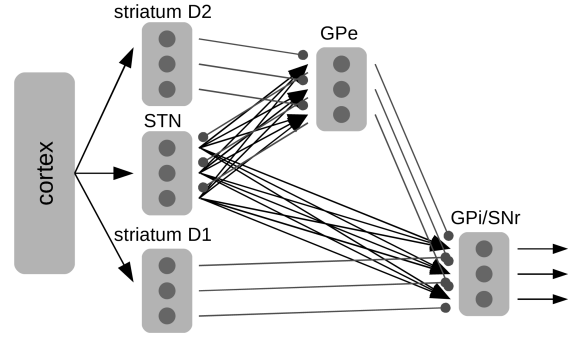
\includegraphics[scale=1]{media/gpr3.png}
	\caption{Simplified basal ganglia model that performs action selection in a scalable manner.}
	\label{fig:simple_bg}
\end{figure}

\subsection{Serial Working Memory}

\begin{figure}[t]
	\centering
	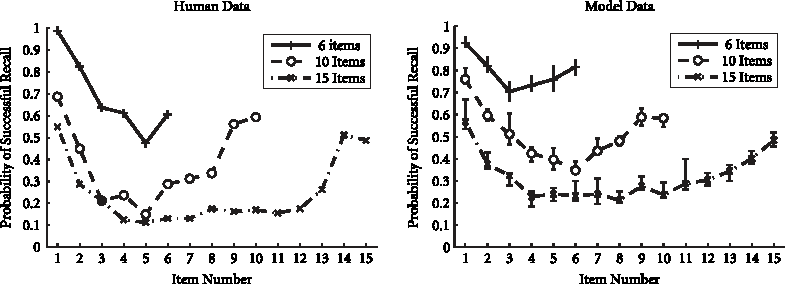
\includegraphics[scale=1.2]{media/htbab_ose_experiment.pdf}
	\caption{Human experimental data on serial recall, as well as the corresponding model-generated data. Figure copied from Eliasmith, \enquote{How to build a brain}, 2013, Figure 6.2. Human data from Jahnke, \emph{Delayed recall and the serial-position effect of short-term memory}, 1986 \cite{jahnke1968delayed}.}
	\label{fig:htbab_ose_experiment}
\end{figure}

\begin{figure}[t]
	\centering
	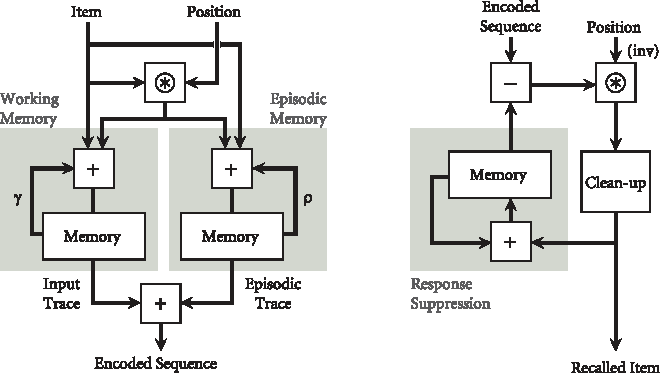
\includegraphics[scale=1.2]{media/htbab_ose.pdf}
	\caption{Ordinal serial encoding model. The left portion of the diagram shows the two sub-memories, responsible for the \enquote{recency} and \enquote{primacy} effects. Figure copied from Eliasmith, \enquote{How to build a brain}, 2013, Figure 6.3.}
	\label{fig:htbab_ose}
\end{figure}

Working memory describes the ability of animals to remember a limited amount of information for immediate processing (colloquially, \enquote{keeping something in mind}). Correspondingly, working memory is typically assumed to span time spans of a couple of seconds, and, is as you might know from personal experience, quite flawed.

Working memory (or, here, synonymously \emph{short-term memory}), has been extensively studied by psychologists in various experiments. One such experiment is delayed serial recall. Participants are presented with a list of random words, one at a time, and are then asked to reproduce the list in order.

When repeating this experiment multiple times with lists of different lengths, one will find that participants are relatively good at remembering the first and last words in the list, but can often not remember the words in between. The ability to remember the initial words is called \emph{primacy effect} (i.e., the first (primal) observations of a new sequence of events are remembered), the ability to remember the last words is called \emph{recency effect} (i.e., the most recent events are still in memory) (\cref{fig:htbab_ose_experiment}).

As we have discussed before, in the context of the NEF, we think about working memory content as being encoded in neural activity patterns and not in neural connection weights. Furthermore, we discussed neural integrators as a kind of working memory. Instead of just representing one dimension, we can also implement higher-dimensional neural integrators that \enquote{remember} entire semantic pointers $\vec x$ (this requires careful tuning of the neural encoders). Changing the amount of feedback in an integrator can give your network more of a recency (<1) or primacy (>1) behaviour (see Nengo example 19 SPA).

When presenting a sequence of symbol vectors $\Obj{ITEM_A}, \Obj{ITEM_B}, \ldots, \Obj{ITEM_X}$, a perfect integrator will automatically remember the sum of these symbol vectors, i.e., the state $\vec x$ after all items have been presented is given as a weighted sum of the individual symbol vectors:
\begin{align*}
	\vec x &= \Obj{ITEM_A} + \Obj{ITEM_B} + \ldots + \Obj{ITEM_X} \,.
\end{align*}
Of course, when building a model of the above experiment, we also need to store the position of the items within the list. As we have discussed in the last lecture, we can use unitary symbol vectors to create an arbitrary long sequence of symbol vectors encoding integer positions
\begin{align*}
	\Obj{POS}_i &= \underbrace{\Obj{POS} \CC \Obj{POS} \CC \ldots \CC \Obj{POS}}_{i \text{ times}} \,, & \text{where } \Obj{POS} \text { is a unitary vector, i.e. } \| \vec x \CC \Obj{POS} \| = \| \vec x \| \,.
\end{align*}
We can thus create these position vectors \enquote{on-the-fly} whenever a new item is presented, by just binding \Obj{POS} to the previous position vector.

Depending on how exactly the integrator is tuned (i.e., whether it is implemented as a leaky integrator or not, what the strength of the feedback connection is, radius of the population, etc.), a neural integrator implemented using NEF principle three can either show recency or primacy effects. Combining a primacy and a recency memory system thus allows us to implement a model of human serial working memory. Having two memory systems maps well onto the human brain, where we know that prefrontal cerebral cortex (PFC) is responsible for representing events in the immediate past, whereas Hippocampus is involved in remembering events in the more distant past (this type of memory is also referred to as \enquote{episodic memory}). See the left half of \cref{fig:htbab_ose} for an overview diagram of this memory model.

Of course, in order to recall items from this memory in series, we need a circuit capable of decoding the sequence. Na\"ively, we can just apply the binding operator to the pseudo-inverse of the position we would like to extract. In order to improve the performance of the system, we can additionally  remember which items were already recalled, and subtract those from the symbol vector encoding the sequence. This system is depicted in the right half of \cref{fig:htbab_ose}.

An experiment comparing human performance to the performance of this memory system is depicted in the right half of \cref{fig:htbab_ose_experiment}. As visible, the model data matches the human performance quite well, both qualitatively and quantitatively.


\Note{\emph{Repeating experiments.} When evaluating NEF models, one should always repeat the experiment several times with different random seeds. This will cause the $x$-intercepts, maximum firing rates and encoders to be different in each trial. Each of these experimental trials can be interpreted as a different \enquote{participant}. One should then look at the distribution of the results, for example by visualising the mean, median, standard deviation, and the 10-/90-percentiles in a box plot (see \href{https://en.wikipedia.org/wiki/Box_plot}{Wikipedia} and \href{https://matplotlib.org/3.1.0/api/_as_gen/matplotlib.pyplot.boxplot.html}{the Matplotlib documentation} for more information).}

\section{Spaun}

\begin{figure}
	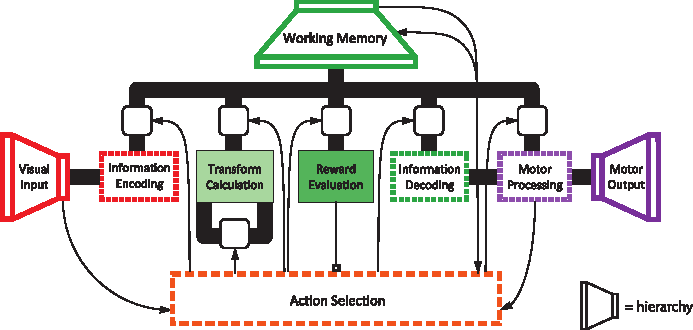
\includegraphics[width=\textwidth]{media/eliasmith_2012_spaun_architecture.pdf}
	\caption{SPAUN's architecture. Visual input and motor output translate visual stimuli into semantic pointers and vice versa. Information is routed to different subsystems according to an action selection system, which, turn, is controlled by the content of the working memory and a reward system. Figure copied from \cite{eliasmith2012largescale}.}
	\label{fig:eliasmith_2012_spaun_architecture}
\end{figure}

\begin{figure}
	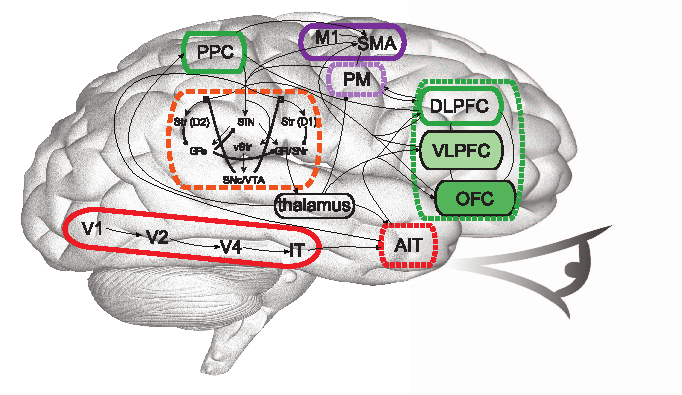
\includegraphics[width=\textwidth]{media/eliasmith_2012_spaun_anatomy.pdf}
	\caption{Brain areas modelled by Spaun. Colours correspond to those found in \cref{fig:eliasmith_2012_spaun_architecture}. The orange dashed line corresponds to the Basal Ganglia. Figure copied from \cite{eliasmith2012largescale}.}
	\label{fig:eliasmith_2012_spaun_anatomy}
\end{figure}

As mentioned above, Spaun is one of the largest functional brain models to date~\cite{eliasmith2012largescale}. Spaun implements the ideas discussed above. Visual input is directly translated into semantic pointers, and semantic pointers representing motor actions are used to drive a motor system (\cref{fig:eliasmith_2012_spaun_architecture}).

Processing---apart from visual input and motor output---consists of a comparably small set of building blocks information is routed to according to an action selection system. The action selection system we saw above is driven by the state of the working memory and a reward evaluation model. All these building blocks are coarsely modelled after individual brain regions, as detailed in \cref{fig:eliasmith_2012_spaun_anatomy}. Although Spaun consists of relatively few modules, it is able to flexibly use these components to solve a variety of tasks---without the experimenter having to intervene and reconfigure the model (see here for some videos showing Spaun in action: \YouTube[digit recognition]{f6Ul5TYK5-o}, \YouTube[copy drawing]{WNnMhF7rnYo}, \YouTube[addition by counting]{mP7DX6x9PX8}, \YouTube[pattern completion]{Q_LRvnwnYp8}). The full playlist is \href{https://www.youtube.com/playlist?list=PLYLu6sY3jnoV2DNi84T5OKqJ0oYTxFrQv}{here} (note these are for Spaun 1, Spaun 2.0 has fewer movies).

For a detailed description of the model, refer to \enquote{How to Build a Brain} \cite{eliasmith2013how}.

\printbibliography

\end{document}

